\documentclass[12pt]{exam}
\usepackage[utf8]{inputenc}

\usepackage[margin=1in]{geometry}
\usepackage{amsmath,amssymb}
\usepackage{multicol}
\usepackage{graphics} % for pdf, bitmapped graphics files
\usepackage{graphicx}
\usepackage{subfigure}
\usepackage{listings}
\usepackage{hyperref}
\lstset{basicstyle=\ttfamily,breaklines=true}
\newcommand{\class}{CS1000 ICC}
\newcommand{\term}{Pregrado}
\newcommand{\examnum}{Práctica Calificada 1}
\newcommand{\examdate}{2021-II}
\newcommand{\timelimit}{110 minutos}
\newcommand{\professor}{Profesor: Francisco Vilchez}
\newcommand{\seccion}{Lab 1.0(1,2)}
\pagestyle{head}
\firstpageheader{}{}{}
\runningheader{CS1000}{\examnum\ - Página \thepage\ de \numpages}{\examdate}
\runningheadrule

\begin{document}
\noindent
\begin{tabular*}{\textwidth}{l l  l}
    \begin{minipage}{1.8in}
        
\includegraphics[width=\textwidth, height=30mm]{logo.png}
    \end{minipage}
    &
    \begin{minipage}{4.7in}
    \begin{flushright}
         \Large \textbf{\class} \normalsize \\
         \large \textbf{\examnum}\\
         \large \textbf{\term}\\
         \large \textbf{\examdate}\\
         \large \textbf{\professor}\\
         \large \textbf{\seccion}
    \end{flushright}
    \end{minipage}
 &\\
\end{tabular*}\\

\rule[2ex]{\textwidth}{2pt}
\Large Indicaciones específicas:
\normalsize
\begin{itemize}
  \item El desarrollo de esta práctica es estrictamente individual.
  \item Esta evaluación contiene \numpages\ páginas (incluyendo esta página) con \numquestions\ preguntas. El total de puntos son \numpoints.
  \item El tiempo límite para la evaluación es \timelimit.
  \item Cada pregunta deberá ser respondida con el nombre de archivo solicitado.
  \begin{enumerate}
    \item\begin{enumerate}
      \item \texttt{pregunta1\_1.png}
      \item \texttt{pregunta1\_2.png}
      \item \texttt{pregunta1\_3.png}
      \item \texttt{pregunta1\_4.png}
    \end{enumerate}
    
    \item \texttt{pregunta2.py}
    \item \texttt{pregunta3.md}
    \item \texttt{pregunta4.sql}
  
  \end{enumerate}

  \item Sólo se corregirá los archivos con dichos nombres. Otro archivo con otro nombre o extensión no será considerado para la calificación.
  % \item Recuerda que el Gradescope solo conserva el último envio que se realiza, por lo tanto una vez que tengas las 4 preguntas resueltas,\textbf{deberás arrastrar los 4 archivos de manera simultánea y subirlos al Gradescope}.\\
  %  \href{https://www.gradescope.com}{www.gradescope.com}
\end{itemize}


% \Large Competencias:
% \normalsize
% \begin{itemize}
% \item Para los alumnos de la carrera de Ciencia de la Computación
% \begin{itemize}
%   \item Aplicar conocimientos de computación y de matemáticas apropiadas para la disciplina. (\textbf{Usar})
% \end{itemize}


% \item Para los alumnos de las carreras de Ingeniería
%   \begin{itemize}
%   \item Capacidad de aplicar conocimientos de ingeniería (\textbf{nivel 2}).
%   \end{itemize}
% \end{itemize}
\newpage
\noindent
\rule[2ex]{\textwidth}{2pt}
\Large{Calificación}:
\normalsize
\begin{center}
Tabla de puntos (sólo para uso del professor)\\
\addpoints
\gradetable[v][questions]
\end{center}
\noindent
\newpage

\begin{questions}

\question[5] Compuertas Lógicas.

En el laboratorio 2 del curso, aprendimos que la computadora utiliza transistores para almacenar los datos sobre los cuales opera. Por esta razón, el procesador se ve en la necesidad del uso de los operadores lógicos AND, OR y NOT para poder realizar operaciones booleanas o aritméticas.

Un ejemplo de un operador matemático es el operador de suma, el cual recibe dos números a operar y devuelve un resultado.

El operador \lstinline{medio sumador} realiza la operación de suma pero de sólo dos bits. Devolviendo un bit de acarreo y un bit de suma. Su tabla de verdad puede ser apreciada en la Figura \ref{fig:suma}:

\begin{figure}[ht!]
  \centering
  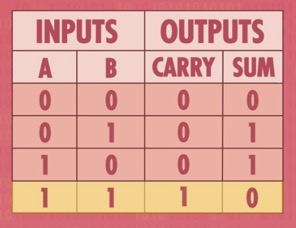
\includegraphics[width=0.4\linewidth]{../figures/suma.jpg}
  \caption{Tabla de verdad del operador \lstinline{medio sumador}}
  \label{fig:suma}
\end{figure}

Donde SUM es la Suma de ambos bits, y CARRY es el acarreo de la suma.

Implemente el operador \lstinline{medio sumador} utilizando \href{https://academo.org/demos/logic-gate-simulator/}{la herramienta online} usada en el laboratorio y únicamente los operadores AND, OR y NOT.

La operación \lstinline{medio sumador} esta representada por la siguiente ecuación:

\begin{displaymath}
  SUM=A\overline{B}\cdot{}B\overline{A}
\end{displaymath}

\begin{displaymath}
  CARRY=A\cdot{}B
\end{displaymath}

\emph{Tip: Empiece analizando la cantidad de entradas y salidas necesarias. Después de ello, empiece a agregar los operadores necesarios. Recuerde que solo puede utilizar los operadores AND, OR y NOT.}

Suba una imagen del circuito para cada uno los casos mostrados en la tabla de verdad, en archivos llamados \lstinline{pregunta1_1.png}, \lstinline{pregunta1_2.png}, \lstinline{pregunta1_3.png} y \lstinline{pregunta1_4.png}.

\newpage

La r\'ubrica para esta pregunta es:

\begin{table}[h]
  \resizebox{\textwidth}{!}{
    \begin{tabular}{|p{0.2\linewidth}|p{0.2\linewidth}|p{0.2\linewidth}|p{0.2\linewidth}|p{0.2\linewidth}|}

    \hline

    \textbf{Criterio} & 
    \textbf{Excelente} & 
    \textbf{Adecuado } & 
    \textbf{Mínimo} & 
    \textbf{Insuficiente} \\ 
    
    \hline

    Uso de compuertas lógicas (3pts) &
    Utiliza correctamente las compuertas lógicas para el circuito solicitado. \textbf{(3pts)}&
    Realiza correctamente el circuito solicitado para SUM, sin embargo, existe un error en las compuertas que calculan el CARRY. \textbf{(2pts)}&
    Realiza correctamente el circuito solicitado para el CARRY, sin embargo, existe un error en las compuertas que calculan el SUM.  \textbf{(1pts)}&
    No calcula correctamente ni el SUM ni el CARRY. \textbf{(0pts)}\\

    \hline

    Identifación de entradas y salidas (2pts) &
    Identifica correctamente la cantidad de entradas y salidas en el circuito. \textbf{(2pts)} &
    Identifica correctalmente la cantidad de entradas, pero no la cantidad de salidas. \textbf{(1pts)} &
    Identifica correctamente la cantidad de salidas, pero no la cantidad de entradas. \textbf{(0.5pts)} &
    No demuestra conocimiento de las entradas y salidas en el circuito. \textbf{(0pts)} \\

    \hline

    \end{tabular}
  }
\end{table}

\newpage

\question[5] Operaciones con bits en Python

En el laboratorio 3, aprendimos algunos operadores a nivel de bits de python. Entre ellos, los operadores:

\begin{itemize}
  \item \lstinline{&}: realiza bit a bit la operación AND en los operandos.
  \item \lstinline{|}: realiza bit a bit la operación OR en los operandos.
  \item \lstinline{^}: realiza bit a bit la operación XOR en los operandos.
\end{itemize}

Se le presenta una función en python llamada \lstinline{numero_unico}. Dicha función recibe 7 números, todos los números están repetidos una vez. \textbf{Sólo uno de ellos no está repetido.}

Se le pide modificar la función \lstinline{numero_unico} de tal manera que guarde en la variable \lstinline{respuesta} el número que no está repetido.

\textbf{Restricción}: Sólo puede utilizar los operadores mencionados. En otras palabras, solo puede utilizar \lstinline{&}, \lstinline{|}, \lstinline{^}.

Tiene permitido utilizar el símbolo \lstinline{=} para asignar el resultado a la variable \lstinline{resultado}.

\begin{lstlisting}[frame = single, language=python, caption=Funcion numero\_unico]]
  def numero_unico(num1,num2,num3,num4,num5,num6,num7):
    # realice aqui sus operaciones
    # respuesta = ...?
    
    print(respuesta)
\end{lstlisting}

Ejemplo 1:

Invocar la funci\'on con los siguiente valores:

\begin{lstlisting}[frame = single, language=python, caption=Ejemplo 1]]
numero_unico(4, 7, 15, 7, 4, 15, 9)
\end{lstlisting}

Retornar\'a:
\begin{lstlisting}[frame = single, language=python, caption=Output 1]]
9
\end{lstlisting}

Ejemplo 2:

Invocar la función con los siguiente valores:

\begin{lstlisting}[frame = single, language=python, caption=Ejemplo 2]]
numero_unico(3, 1, 1, 4, 4, 3, 5)
\end{lstlisting}
Retornará:
\begin{lstlisting}[frame = single, language=python, caption=Output 2]]
5
\end{lstlisting}

Suba su respuesta en un archivo llamado \lstinline{pregunta2.py}.



\newpage

La r\'ubrica para esta pregunta es:

\begin{table}[h]
  \resizebox{\textwidth}{!}{
    \begin{tabular}{|p{0.2\linewidth}|p{0.2\linewidth}|p{0.2\linewidth}|p{0.2\linewidth}|p{0.2\linewidth}|}

    \hline

    \textbf{Criterio} & 
    \textbf{Excelente} & 
    \textbf{Adecuado } & 
    \textbf{Mínimo} & 
    \textbf{Insuficiente} \\ 
    
    \hline

    Desarrollo del código en Python (5pts) &
    El código funciona correctamente e imprime la respuesta con el comando indicado. \textbf{(5pts)} &
    El código funciona correctamente, sin embargo no imprime la respuesta con el comando indicado. \textbf{(4pts)} &
    El código funciona correctamente, utiliza adecuadamente las funciones binarias, sin embargo no devuelve la respuesta esperada. \textbf{(0.5pts)} &
    No realizó procedimiento alguno. \textbf{(0pts)}\\

    \hline

    \end{tabular}
  }
\end{table}


\newpage

\question[5] Git

En el laboratorio 4 aprendimos a utilizar el \href{https://docs.github.com/en/github/writing-on-github/getting-started-with-writing-and-formatting-on-github/basic-writing-and-formatting-syntax}{Markdown de GitHub} para crear nuestro archivo README en nuestra página de GitHub. Se le pide que replique el archivo ubicado en la siguiente página utilizando en Markdown de GitHub.

Puede obtener la imagen del siguiente \href{https://preview.redd.it/sk9nb6lgccq31.gif?format=png8&s=4314adede1e763a54cb4b435e3d246da0460d3ae}{link}

Donde necesite especificar algún link, puede utilizar cualquier URL.

No utilice \lstinline{HTML}. Sólo puede utilizar el Mardown de GitHub.

Suba su archivo como \lstinline{pregunta3.md}

\newpage

\begin{figure}[ht!]
  \centering
  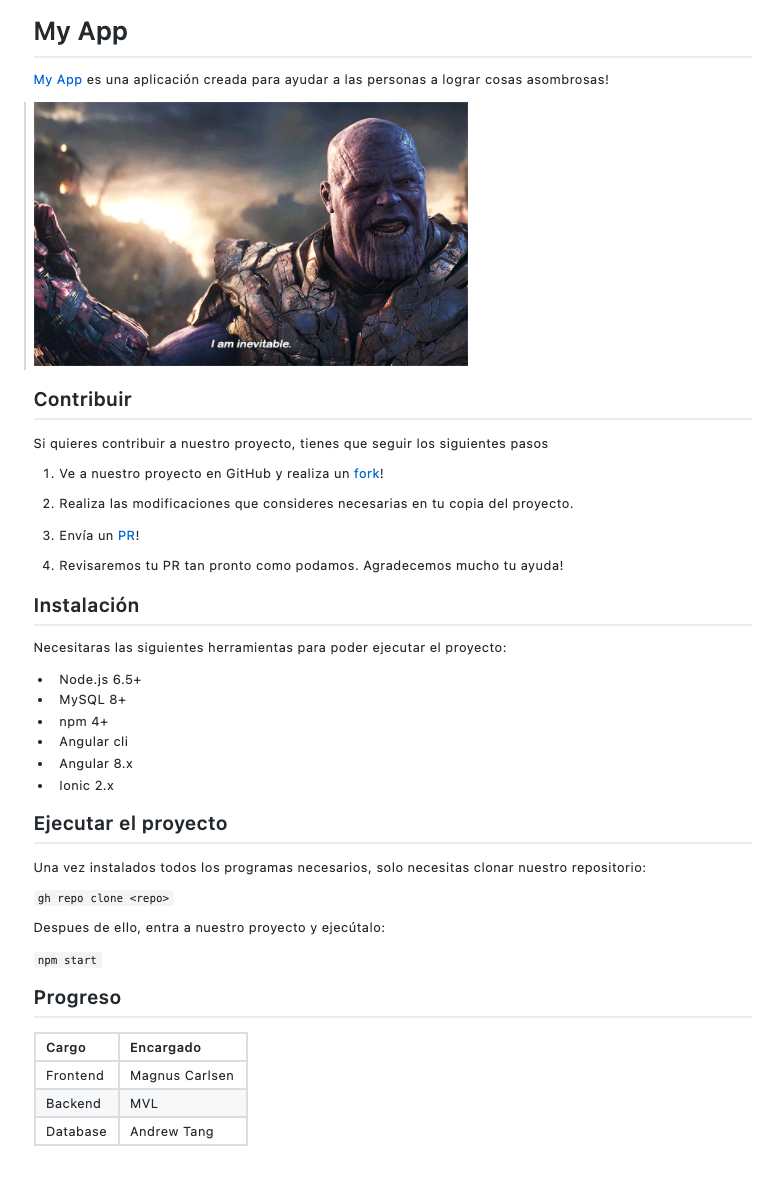
\includegraphics[width=0.9\linewidth]{../figures/pregunta3.png}
  \label{fig:p3}
\end{figure}

\newpage

La rúbrica para esta pregunta es:

\begin{table}[h]
  \resizebox{\textwidth}{!}{
    \begin{tabular}{|p{0.2\linewidth}|p{0.2\linewidth}|p{0.2\linewidth}|p{0.2\linewidth}|p{0.2\linewidth}|}

    \hline

    \textbf{Criterio} & 
    \textbf{Excelente} & 
    \textbf{Adecuado } & 
    \textbf{Mínimo} & 
    \textbf{Insuficiente} \\ 
    
    \hline

    Uso de títulos y subtítulos (1pts) &
    Identifica y utiliza adecuadamente títulos y subtítulos donde corresponde. \textbf{(1pts)} &
    Usa adecuandamente títulos, sin embargo no identifica subtítulos. \textbf{(0.75pts)}&
    Usa adecuandamente títulos y subtítulos, sin embargo, faltó incluir un título/subtítulo de los solicitados. \textbf{(0.25pts)}&
    No demuestra conocimiento del uso de títulos o subtítulos. \textbf{(0pts)}\\
    
    \hline

    Creación de tablas (1pts) &
    Realiza correctamente la creación de la tabla solicitada. \textbf{(1pts)}&
    Realiza la creación de la tabla sin definir correctamente la cabecera de la tabla. \textbf{(0.75pts)}&
    Realiza la creación de la tabla, sin embargo no incluye todas las filas o columnas solicitadas. \textbf{(0.25pts)}&
    No demuestra conocimiento del uso adecuado de tablas. \textbf{(0pts)}\\

    \hline

    Creación de listas enumeradas y sin enumerar (1pts) &
    Realiza correctamente la creación de listas enumeradas y sin enumerar. \textbf{(1pts)} &
    Realizar correctamente la creación de listas enumeradas y sin enumerar, pero no toda la información solicitada. \textbf{(0.5pts)} &
    Realiza la creación de listas enumeradas pero no las sin enumerar, o viceversa. \textbf{(0.25pts)} &
    No demuestra conocimiento de listas enumeradas y sin enumerar. \textbf{(0pts)}\\

    \hline

    Creación de links, bloques de codigo (1pto) &
    Realiza correctamente la creación de links y bloques de código. \textbf{(1pts)} &
    Realizar correctamente la creación de links y bloques de código, pero notoda la información solicitada. \textbf{(0.5pts)} &
    Realiza la creación de links pero no los bloques de código, o viceversa. \textbf{(0.25pts)} &
    No demuestra conocimiento de links y bloques de código. \textbf{(0pts)}\\

    \hline

    Inclusión de imágenes y texto (1pts) &
    Realiza correctamente la creación imagénes y el texto solicitado\textbf{(1pts)} &
    Realizar correctamente la creación de la imágen, sin embargo el archivo no tiene todo el texto requerido \textbf{(0.5pts)} &
    No realiza correctamente la creación de la imagen, pero el archivo tiene el resto del texto \textbf{(0.25pts)} &
    No demuestra conocimiento de inclusión de imágenes ni de texto plano. \textbf{(0pts)}\\
    
    \hline

    \end{tabular}
  }
\end{table}

\newpage

\question[5] SQL

En el laboratorio 6 aprendimos a utilizar SQL para la creación de tablas en una \href{https://extendsclass.com/mysql-online.html}{Base de Datos online}.

El Gobierno del Perú desea realizar la creación de una base de datos para almacenar la información de las personas que se han vacunado, y los detalles de las dosis que recibieron.

Se le pide para ello, con los siguientes detalles:

\begin{enumerate}
  \item Crear una tabla llamada \lstinline{persona_vacunada}. Debe almacenar la siguiente información
  
  \begin{itemize}
    \item Nombre completo (Campo obligatorio)
    \item Género (Campo opcional)
    \item Email (Campo opcional)
    \item Nombre de la vacuna (Campo obligatorio)
    \item Cantidad de dosis (Campo obligatorio)
  \end{itemize}

  Usa una columna \lstinline{id} como llave primaria, esta debe incrementarse con cada inserción.

  \item Crear las sentencias \lstinline{INSERT} para ingresar los siguientes datos a la base de datos:
  
  \begin{itemize}
    \item La persona con nombre Francisco Vilchez de género Masculino ha recibido 2 dosis de la vacuna Pfizer. No ha especificado email.
    \item La persona con nombre Mauree Turner recibió 2 dosis de la vacuna Sinopharm. No especificó género, pero indicó que su correo es mauree@turner.com
    \item La persona con nombre Rameshbabu Praggnanandhaa recibió 2 dosis de la vacuna Covaxin. No especificó su genero ni su correo.

  \end{itemize}

\end{enumerate}

Suba sus comandos en el orden en que deben ser ejecutados en el archivo \lstinline{pregunta4.sql}

\newpage

La rúbrica para esta pregunta es:

\begin{table}[h]
  \resizebox{\textwidth}{!}{
    \begin{tabular}{|p{0.2\linewidth}|p{0.2\linewidth}|p{0.2\linewidth}|p{0.2\linewidth}|p{0.2\linewidth}|}

    \hline

    \textbf{Criterio} & 
    \textbf{Excelente} & 
    \textbf{Adecuado} & 
    \textbf{Mínimo} & 
    \textbf{Insuficiente} \\ 
    
    \hline

    Creación de tablas (2pts) &
    Realiza la creación de la tabla utilizando el comando adecuado, con los atributos necesarios para guardar la información solicitada y respectivos tipos de datos adecuados. \textbf{(2 pts)} & 
    Realiza la creación de la tabla utilizando el comando adecuado con los tipos de dato adecuados, sin embargo, los atributos utilizados no permiten almacenar la información en su totalidad. \textbf{(1 pts)}&
    Realiza la creación de la tabla utilizando el comando adecuando, sin embargo los atributos utilizados y los tipos de datos usados son incorrectos ya que no permiten almacenar la información solicitada. \textbf{(0.5 pts)}&
    No demuestra conocimiento de la sintaxis del comando para la creación de tablas. \textbf{(0 pts)} \\

    \hline

    Inserción de datos (3pts) &
    Realiza la correcta inserción de cada uno de los datos solicitados. \textbf{(3 pts)}&
    Realiza correctamente inserción de alguno de los datos solicitados. \textbf{(2 pts)}&
    El comando de inserción de datos tiene la sintaxis correcta, sin embargo los tipos de datos utilizados o el orden de ellos no va conforme con la estructura de la tabla. \textbf{(1 pts)}&
    No demuestra conocimiento de la sintaxis del comando para la inserción de datos. \textbf{(0 pts)}\\

    \hline
    \end{tabular}
  }
\end{table}

\end{questions}

\end{document}
